\documentclass[dvipdfmx,tikz]{standalone}
\usepackage{tikz}
\usepackage{ifthen}


\usetikzlibrary{
  shapes,
  shapes.geometric,
  arrows.meta,
  calc,
}

\definecolor{cA}{HTML}{0072BD}
\definecolor{cB}{HTML}{EDB120}
\definecolor{cC}{HTML}{77AC30}
\definecolor{cD}{HTML}{D95319}

\begin{document}
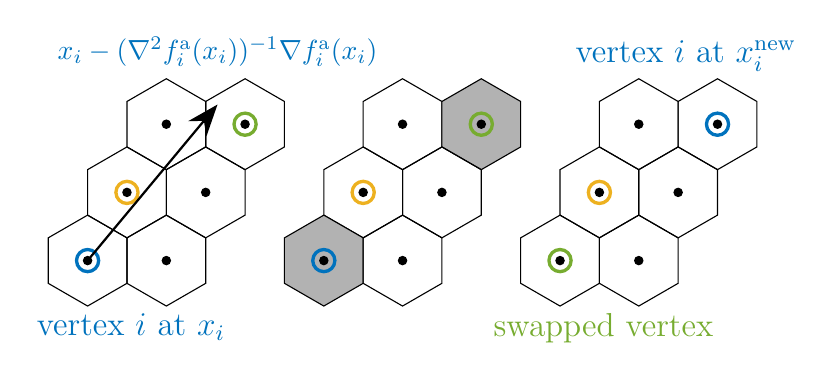
\begin{tikzpicture}
  \foreach \X in {0,1,2}{
      \begin{scope}[xshift=3*\X cm]
        \foreach \x in {0,1,2}{
            \foreach \y in {0,1}{
                \pgfmathsetmacro\shift{mod(\x,2)*0.5+max(\x-1,0)}
                \coordinate (a\x\y) at ({\y - \shift},{-sqrt(3)/2*\x});
              }}

        \foreach \x in {0,1,2}{
            \foreach \y in {0,1}{
                \ifthenelse{
                  \(\X=1 \AND \x=0 \AND \y=1\) \OR
                  \(\X=1 \AND \x=2 \AND \y=0\)
                }{
                  \node[regular polygon, regular polygon sides=6, minimum size=1.1547005cm, draw,rotate=30,fill=black!30!white] at (a\x\y) {};
                }{
                  \node[regular polygon, regular polygon sides=6, minimum size=1.1547005cm, draw,rotate=30] at (a\x\y) {};
                }
                \filldraw[draw=black,fill=black] (a\x\y) circle (1.5pt);
              }
          }

        \ifthenelse{\X=0 \OR \X=1}{
          \draw[cA,very thick] (a20) circle (4pt);
          \draw[cB,very thick] (a10) circle (4pt);
          \draw[cC,very thick] (a01) circle (4pt);
        }{
          \draw[cA,very thick] (a01) circle (4pt);
          \draw[cB,very thick] (a10) circle (4pt);
          \draw[cC,very thick] (a20) circle (4pt);
        }

        \ifthenelse{\X=0}{
        \draw[thick,-{Stealth[length=4mm]}] (a20) -- ($(a01)+(-0.35,0.25)$) node[above=0.35cm,cA] {$x_i-(\nabla^2 f^\mathrm{a}_i(x_i))^{-1}\nabla f^\mathrm{a}_i(x_i)$};

        \node[cA] at (a20)[right=0.55cm, below=0.55cm] {\large vertex $i$ at $x_i$};
        }{}

        \ifthenelse{\X=2}{
          \node[cC] at (a20)[right=0.55cm, below=0.55cm] {\large swapped vertex};

          \node[cA] at (a01)[left=0.4cm,above=0.55cm] {\large vertex $i$ at $x_i^\mathrm{new}$};
        }{}
      \end{scope}
    }
\end{tikzpicture}
\end{document}
